For non-isothermal air flow we have to consider pressure and temperature dependencies of air viscosity $\mu(p, T)$ (section \ref{sec:Reichenberg_viscosity_model}), specific heat capacities $c_p(p, T)$ and heat conductivities $\lambda(p, T)$ (section \ref{sec:thermal_properties}) as well (\cite{McDermottEtAl:2006}).
\subsection{Air dynamic viscosity}
\label{sec:Reichenberg_viscosity_model}
The Reichenberg viscosity model (\cite{ReidEtAl:1988}) is used for the non-isothermal flow of air. The pressure and temperature dependencies of air viscosity are shown in Fig. \ref{fig:visco7}.
\begin{eqnarray}
\mu (p, T)=\mu_0 (T)\left(1 + \frac{A p_r^{\frac{3}{2}}}{B p_r+\left(1+C p_r^D\right)^{-1}}
\right)
\label{eqn:reichenberg_viscosity}
\end{eqnarray}
with the following parameters:
\begin{eqnarray}
\begin{array}{ll}
p_r = \frac{p}{p_{\mathrm {crit}}}
&
T_r = \frac{T}{T_{\mathrm {crit}}}
\\
A = \frac{\alpha_1}{T_r} \exp (\alpha_2 T_r^a)
&
B = A(\beta_1 T_r - \beta_2)
\\
C =\frac{\gamma_1}{T_r} \exp (\gamma_2 T_r^c)
&
D = \frac{\delta_1}{T_r} \exp (\delta_2 T_r^d)
\end{array}
\\
\begin{array}{lll}
p_{\mathrm {crit}} = 33.9 \times 10^4 \mathrm {Pa}
&
T_{\mathrm {crit}} = 126.2 \mathrm {K}
\\
\alpha_1 = 1.9824\times 10^{-3}  &  \alpha_2 = 5.2683  &  a = -0.5767 \\
\beta_1  = 1.6552               &  \beta_2  = 1.2760  &  \\
\gamma_1 = 0.1319                &  \gamma_2 = 3.7035  &  c = -79.8678 \\
\delta_1 = 2.9496                &  \delta_2 = 2.9190  &  d = -16.6169
\end{array}
\nonumber
\end{eqnarray}

% *** EPS-Grafik ***
\begin{figure}[htb!]
\begin{center}
\footnotesize
%\psfrag{Synonym}[pos][pos]{Tex-Ersetzung}
%\psfrag{x}[][]{$t$}
%\psfrag{y}[b][t]{$y(t)$}
%\psfrag{t}[][]{ }
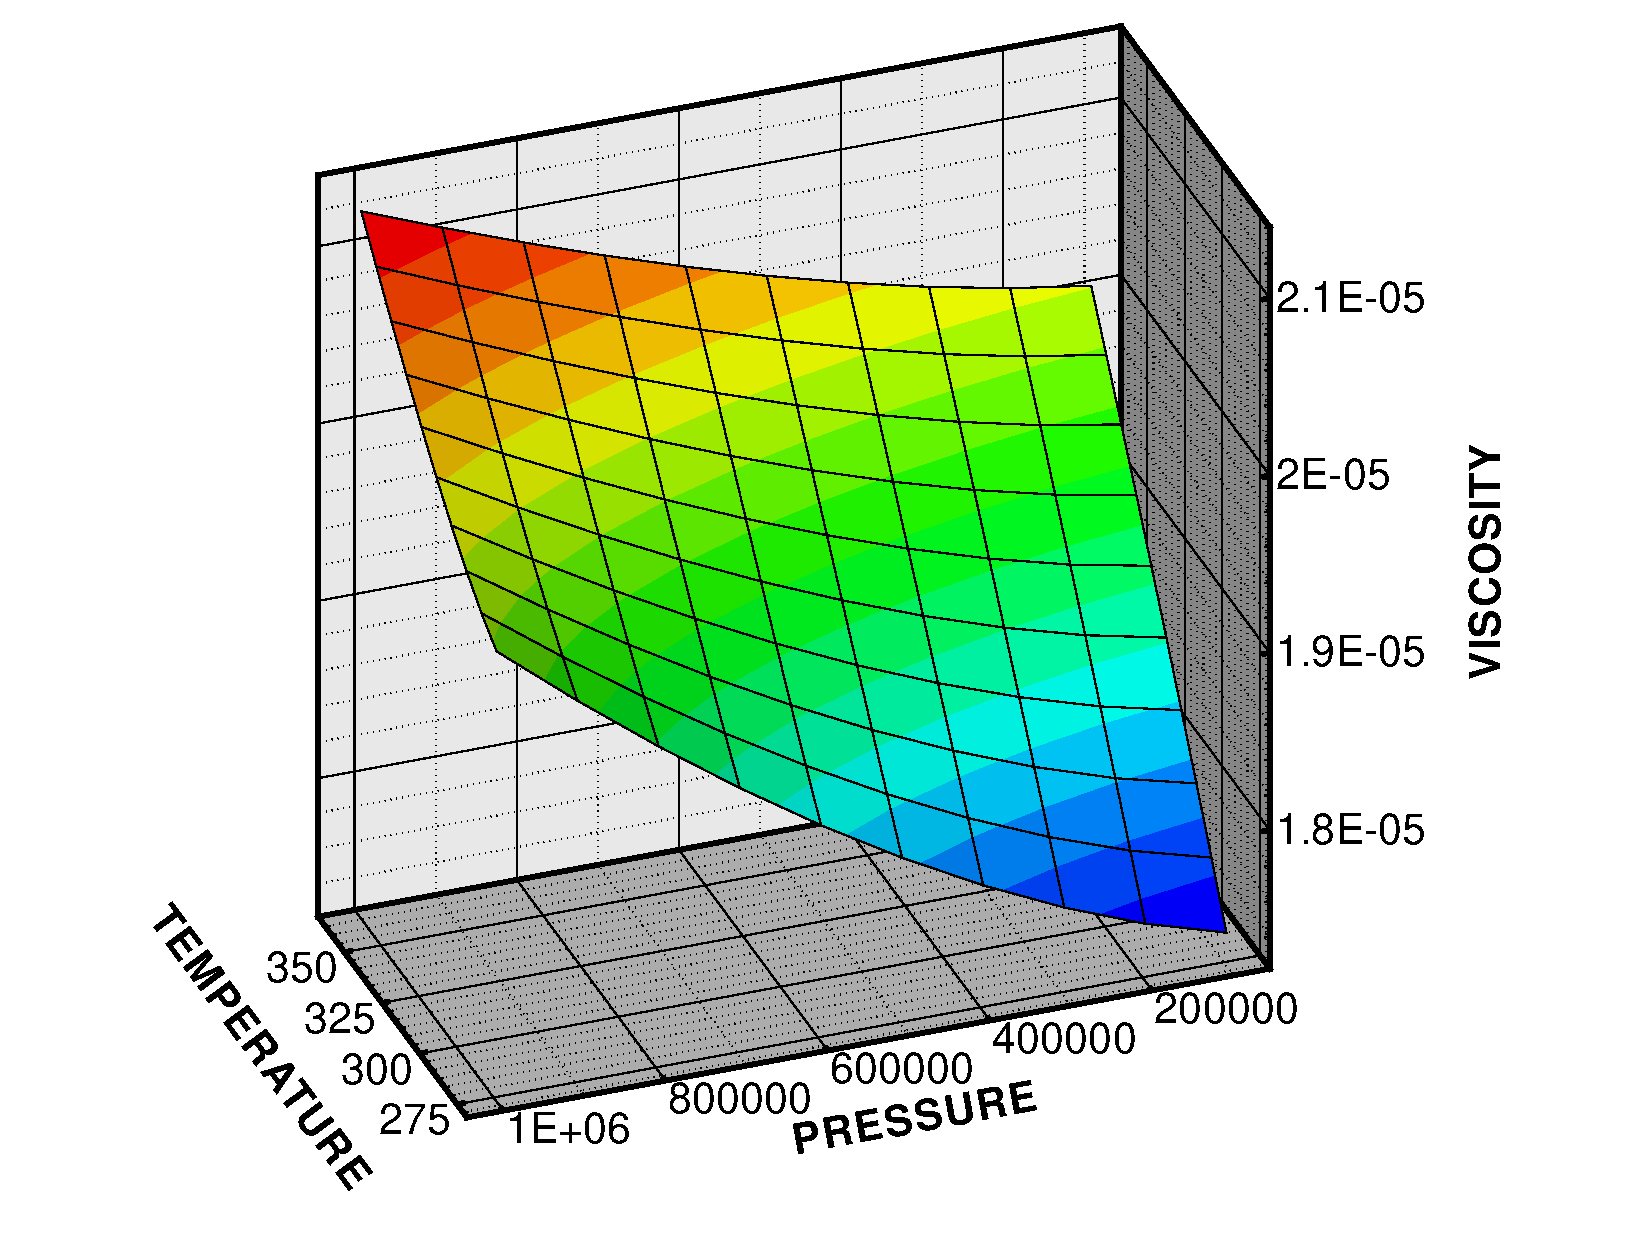
\includegraphics[width=0.6\columnwidth]{PART_II/G/viscosity.eps}  % Filename.eps
\caption{Air viscosity as a function of temperature (in Kelvin) and pressure (in Pa).}
\label{fig:visco7}
\end{center}
\end{figure}

\subsection{Thermal properties}\label{sec:thermal_properties}
\vspace{-0.3cm}Beside the flow characteristics such as air viscosity, the thermal properties, such as heat capacity and thermal conductivity of gas and solid are important for heat transport. As an example, Fig. \ref{fig:thermal_properties} depicts the thermal properties of the gas.
Fig. \ref{fig:thermal_properties} (left) shows the temperature dependence of specific heat capacity of air at atmospheric pressure corresponding to equation (\ref{eqn:heat_capacity}) from \cite{ZografosEtAl:1987} and compared with experimental data by \cite{VargaftikEtAl:1996}. Fig. \ref{fig:thermal_properties} (right) illustrates the temperature dependence of thermal conductivity of air at atmospheric pressure corresponding to equation (\ref{eqn:thermal_conductivity}) from \cite{ZografosEtAl:1987} and compared with experimental data by \cite{VargaftikEtAl:1996}. The pressure dependency of thermal properties can be neglected in the present pressure regimes.
\begin{align}
c_p=a_0+a_1 T+a_2 T^2+a_3 T^3+a_4 T^4
\label{eqn:heat_capacity}
\end{align}
where coefficients $a_0=1.0613$; $a_1=-4.3282 \times 10^{-4}$; $a_2=1.0234 \times 10^{-6}$; $a_3=-6.4747 \times 10^{-10}$; $a_4=1.3864 \times 10^{-13}$.
\begin{align}
\lambda=b_0+b_1 T+b_2 T^2+b_3 T^3+b_4 T^4+b_5 T^5
\label{eqn:thermal_conductivity}
\end{align}
where coefficients $b_0=7.488 \times 10^{-3}$; $b_1=-1.7082 \times 10^{-4}$; $b_2=2.3758 \times 10^{-7}$; $b_3=-2.2012 \times 10^{-10}$; $b_4=9.46 \times 10^{-14}$; $b_5=-1.579 \times 10^{-17}$. 
\begin{figure}[htb!]
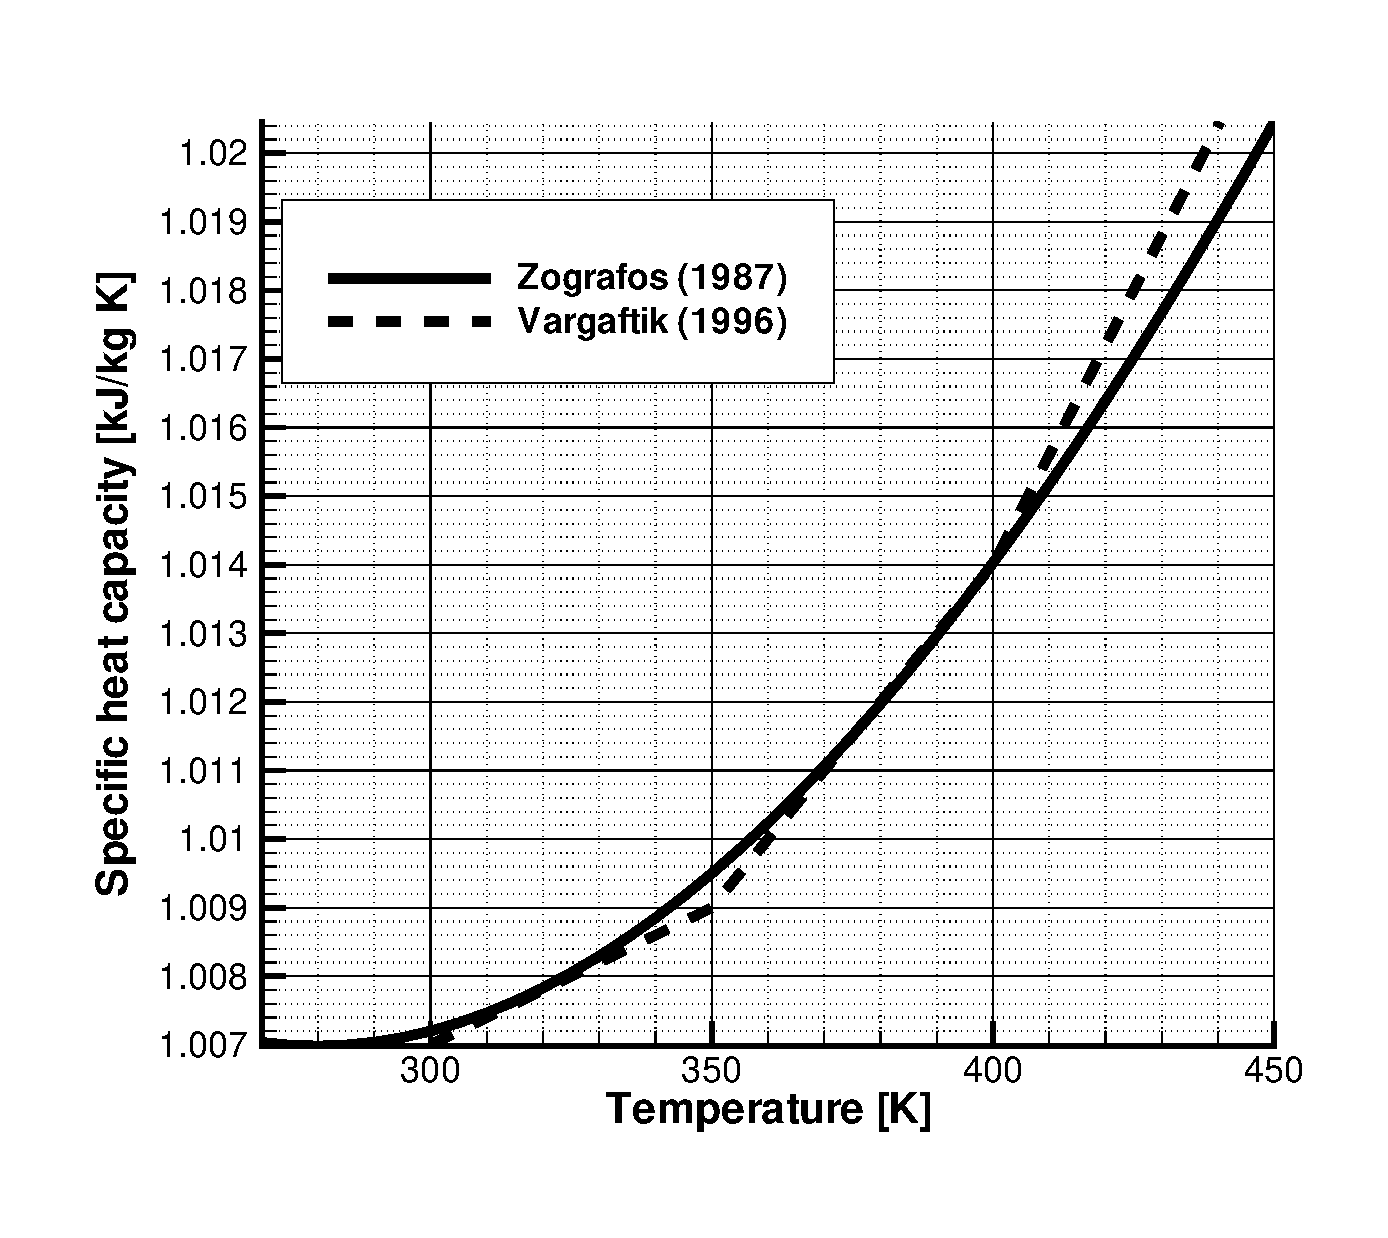
\includegraphics[scale=0.3]{PART_II/G/heat_capacity_air.eps}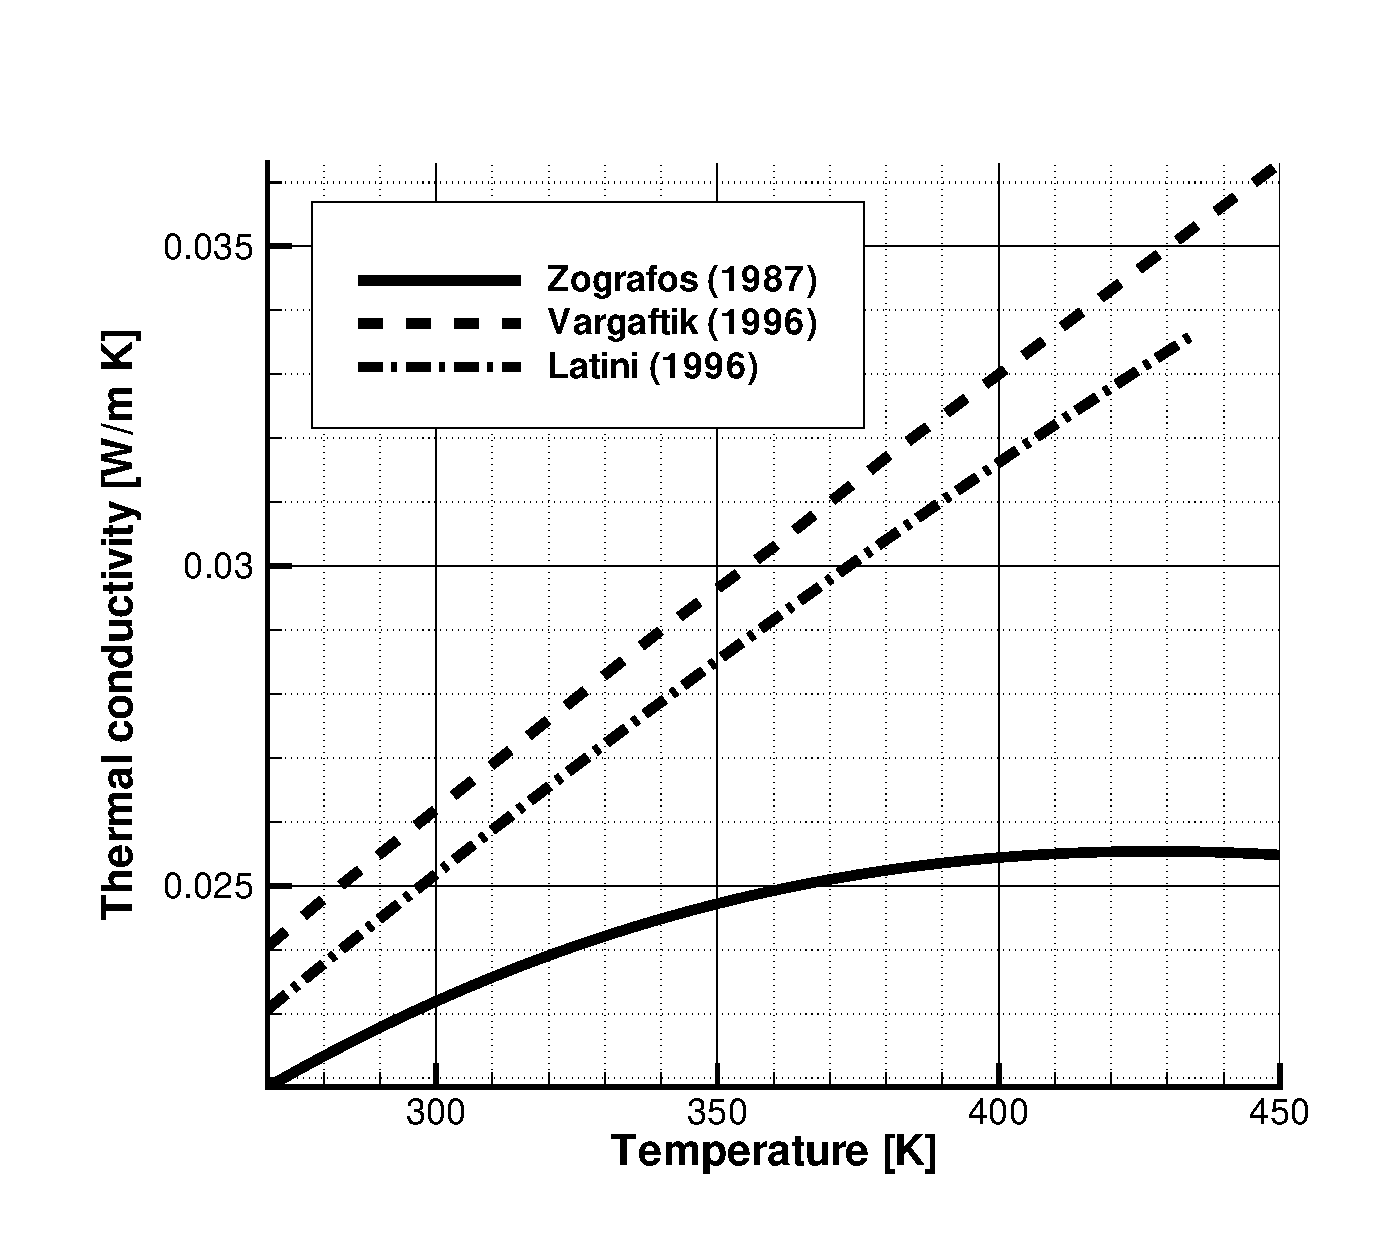
\includegraphics[scale=0.3]{PART_II/G/heat_conductivity_air.eps}
\caption{Thermal properties of air: specific heat capacity (left), thermal conductivity (right).}
\label{fig:thermal_properties}
\end{figure}